%\documentclass[hyperref={pdfpagelabels=false}]{beamer}
\documentclass{beamer}
\DeclareGraphicsExtensions{.pdf,.jpg,.eps,.png}
\definecolor{grisbleu}{rgb}{0.85,0.85,1}
\mode<beamer>{%
 \beamertemplatesolidbackgroundcolor{grisbleu}
  %\usetheme{Hannover}
   %\usetheme{Madrid}
   \usetheme[secheader]{Boadilla}
%   \usetheme[secheader]{Madrid}
%  \usetheme{Pittsburgh}
 \usefonttheme{serif,professionalfonts}
}

\mode<trans>{\usetheme{Pittsburgh}}
%%%%%%%%%%%%%%%%%%%%%%%%%%%%%%%%%%%%%%%%%%%%%%%%%%%%%%%%%%%%%%%%%

%\DeclareGraphicsRule{*}{mps}{*}{} % Figures MetaPost

\usepackage{pgf}

%\usepackage{pdfcolmk}

% Options pour hyperref.sty
\hypersetup{pdfnewwindow=false}
%\hypersetup{pdfpagemode=FullScreen}
\setbeamercovered{dynamic}
  \setbeamertemplate{background canvas}[vertical shading][bottom=red!10,top=blue!10]

\usepackage{amsfonts,amsmath,amssymb,bbm,txfonts,epsfig,epsf,psfrag,color}
%\usepackage[nolists]{endfloat}
\usepackage{enumerate}
%\usepackage{rotate, graphics, epsfig, pstcol}
%\usepackage{/Latex/astats}
\usepackage[english]{babel}
%\usepackage{shortcuts}

\usepackage{xmpmulti}
\usepackage[latin1]{inputenc}
\usepackage[T1]{fontenc}
%\usepackage[oldstyle,upright]{fourier}
\usepackage[upright]{fourier}% Si on n'a pas les compl\'{e}ments expert...
% sf = helvetica scaled 88%
\usepackage[scaled=.88]{helvet}
% tt = lmtt
\renewcommand{\ttdefault}{lmtt}
\newcommand{\textred}[1]{\textcolor{red}{#1}}
\newcommand{\textgreen}[1]{\textcolor{green}{#1}}
\newcommand{\textblue}[1]{\textcolor{blue}{#1}}
\newcommand{\textbrown}[1]{\textcolor{brown}{#1}}
%\newcommand{\textolive}[1]{\textcolor{olive}{#1}}
%\newcommand{\textgray}[1]{\textcolor{gray}{#1}}


%Rajout du package multicol
\usepackage{multicol}
\usepackage[all]{xy}
\usepackage{graphicx}
\beamertemplatenavigationsymbolsempty

\newenvironment{disarray}%
{\everymath{\displaystyle\everymath{}}\array}%
{\endarray}

\renewcommand{\ttdefault}{lmtt}
\newcommand\M{\mathcal{M}}
\newcommand\Lv{\mathcal{L}}
\newcommand\E{\mathbb{E}}
\newcommand\la{\ln{\bf \alpha}}
\newcommand{\Xcal}{\mathcal{X}}
\newcommand{\Zbf}{{\bf Z}}
\newcommand{\Vbf}{{\bf V}}
\newcommand{\Xbf}{{\bf X}}
\newcommand{\Zcal}{\mathcal{Z}}
\newcommand{\wbf}{{\bf w}}
\newcommand{\alphabf}{\text{\mathversion{bold}{$\alpha$}}}
\newcommand{\pibf}{\mbox{\mathversion{bold}{$\pi$}}}
\newcommand{\Pibf}{\mbox{\mathversion{bold}{$\Pi$}}}
\newcommand{\thetabf}{\mbox{\mathversion{bold}{$\theta$}}}
\newcommand{\Thetabf}{\mbox{\mathversion{bold}{$\Theta$}}}
\newcommand{\taubf}{\mbox{\mathversion{bold}{$\tau$}}}
\newcommand{\tah}{\widehat{\tau}}
\newcommand{\tahn}{\tah_{[n]}}
\newcommand{\pibar}{\bar{\pi}}
\newcommand{\Qcal}{\mathcal{Q}}
\newcommand{\RX}{\mathcal{R}_{X}}
\newcommand{\Lcal}{\mathcal{L}}
\renewcommand{\ttdefault}{lmtt}
\newcommand{\Abf}{{\bf A}}
\newcommand{\Bcal}{\mathcal{B}}
\newcommand{\C}{C}
\newcommand{\Esp}{\mathbb{E}}
\newcommand{\eps}{\varepsilon}
\newcommand{\epsbar}{\overline{\eps}}
\newcommand{\etabar}{\overline{\eta}}
\newcommand{\fbf}{{\bf f}}
\newcommand{\Gcal}{\mathcal{G}}
\newcommand{\Hbf}{{\bf H}}
\newcommand{\Ibb}{\mathbb{I}}
\newcommand{\Kcal}{\mathcal{K}}
\newcommand{\lambdabar}{\overline{\lambda}}
\newcommand{\Mcal}{\mathcal{M}}
\newcommand{\Ncal}{\mathcal{N}}
\newcommand{\Pcal}{\mathcal{P}}
\newcommand{\rhobar}{\overline{\rho}}
\newcommand{\Sbf}{{\bf S}}
\newcommand{\Vcal}{\mathcal{V}}
\newcommand{\Vsf}{\mathsf{V}}

\newcommand{\biz}{\begin{itemize}}
\newcommand{\eiz}{\end{itemize}}
\newcommand{\bcent}{\begin{center}}
\newcommand{\ecent}{\end{center}}
\newcommand{\barr}{\begin{array}}
\newcommand{\earr}{\end{array}}
\newcommand{\btab}{\begin{tabular}}
\newcommand{\etab}{\end{tabular}}
\newcommand{\ben}{\begin{enumerate}}
\newcommand{\een}{\end{enumerate}}
\newcommand{\bdes}{\begin{description}}
\newcommand{\edes}{\end{description}}
\newcommand{\dps}{\displaystyle}

\newcommand{\bqas}{\begin{eqnarray*}}
\newcommand{\eqas}{\end{eqnarray*}}
\newcommand{\noi}{\noindent}

%%%% raccourcis Alain

%% Espaces mesurables
%\newcommand{\Z}{\mathcal{Z}}
\newcommand{\Zdefn}{\mathcal{Z}_{n}}
\newcommand{\Xdefn}{\mathcal{X}_{n}}
%\newcommand{\A}{\mathcal{A}}% tribu sur Z
\newcommand{\An}{\mathcal{A}_{n}}
\newcommand{\F}{\mathcal{F}}% tribu sur X
\newcommand{\Fn}{\mathcal{F}_{n}}
\newcommand{\T}{\mathcal{T}}% tribu sur les mesures de proba

%% Points
\newcommand{\Xn}{X_{[n]}}
\newcommand{\xn}{x_{[n]}}
\newcommand{\Zn}{Z_{[n]}}
\newcommand{\zn}{z_{[n]}}
\newcommand{\taun}{\tau_{[n]}}

%% Operateurs
\renewcommand{\L}{\mathcal{L}}
\newcommand{\J}{\mathcal{J}}
\newcommand{\znh}{\widehat{z}_{[n]}}
\newcommand{\zh}{\widehat{z}}
\renewcommand{\th}{\widehat{\tau}}
\newcommand{\tnh}{\widehat{\tau}_{[n]}}
\newcommand{\znt}{\widetilde{z}_{[n]}}

\newtheorem{Prop}{Proposition}
\newtheorem{Propri}{Propri\'et\'es}
\mode<beamer>

\title[Consistency of Variational estimates]{Consistency of Variational estimates for random graphs}
\author[JJ Daudin \& A Celisse]{Jean-Jacques Daudin\inst{1} and Alain Celisse\inst{2}}


\institute{ UMR 518 AgroParisTech/INRA \and UMR 8524 CNRS -- Univ. Lille 1}


\begin{document}
\def\colorize<#1>{\temporal<#1>{\color{black!30}}{\color{red}}{\color{black}}}

%---------------------------------
% Titre
%---------------------------------

\begin{frame}
\titlepage

%\includegraphics[height=1.1cm ] {logagroptech.png} \\

\end{frame}

%---------------------------------
% Introduction
%---------------------------------
%\begin{frame}
%\tableofcontents[]
%\end{frame}

\section{Introduction}
\begin{frame}
\frametitle{Networks}
\begin{description}
  \item[Social networks] phone calls, emails, co-authorship , facebook, influence
  \item[Physical networks] communication, energy
  \item[Ecological networks] trophic, parasitic, mutualistic
  \item[Molecular Biology networks] regulation, PPI, metabolic
\end{description}

\alert {An unusual data set structure}

\begin{tabular}{cc}

  % after \\: \hline or \cline{col1-col2} \cline{col3-col4} ...
  Usual i.i.d. structure & \hspace{1cm} \alert{Structure for networks} \\

  \begin{tabular}{|c|c|c|c|c|}
    \hline
    % after \\: \hline or \cline{col1-col2} \cline{col3-col4} ...
    item &$X_1$ & ... & ... & $X_p$\\
    \hline
    1 & $x_{11}$ & ... & ... & $x_{1p}$ \\
    2 & $x_{21}$ & ... & ... & $x_{2p}$ \\
    . & . & . & . & . \\
    $n$ & $x_{n1}$ & ... & ... & $x_{np}$ \\
    \hline
  \end{tabular}
     &
    \hspace{1cm} \alert{
\begin{tabular}{|c|c|c|}
    \hline
    item1 & item2 & $R$ \\
    \hline
    1 & 2 & $r_{12}$  \\
    1 & 3 & $r_{13}$ \\
    . & . & .  \\
    $n-1$ & $n$ & $r_{n-1,n}$  \\
    \hline
  \end{tabular}
  }
  \\
\end{tabular}

\begin{itemize}
    \item  information is the relation
between two items.
    \item lines  not independent
    \item asymptotic is changed: $n^2$ observations
\end{itemize}

\end{frame}



\begin{frame}
\frametitle{Example: Transcriptional regulatory network of E. Coli}
\begin{tabular}{p{7cm}p{4cm}}
  \hspace{-1.5cm}
\includegraphics[scale=0.30] {Colinet_base.png} &
\vspace{-6cm}\begin{itemize}
    \item nodes are operons
    \item edges between 2 operons if one regules the other
    \item known properties: sparseness, no feed-back circuits, hierarchical organization.
\end{itemize}
{\tiny Data from Shen-Or et al. Nature genetics, 2002}  \\
\end{tabular}

\end{frame}


\begin{frame}
\frametitle{Mixnet}

Mixture model for Bernoulli random graphs:
\begin{itemize}
\item$i=1,n$ nodes
\item $q=1,Q$ classes
\item $X_{ij}=1$ if there is an edge from node $i$ to node $j$.
\item $Z=(Z_1,Z_2,...Z_{n})$ independent discrete latent variable, $Z_{i}=q$ if node $i$ belongs to class $q$
\item $Z_i \sim \Mcal(1,\alpha_1,\alpha_2,...\alpha_Q)$
\item Conditionally to $Z$, $X_{ij}$ are independent Bernoulli RV with
      $$P(X_{ij}=1/Z_i=q,Z_j=l)=\pi_{ql}$$
\end{itemize}
\end{frame}



\begin{frame}
\frametitle{Mixnet results for RTN of E. Coli}
\begin{tabular}{p{5cm}p{6cm}}
  \vspace{0cm}
 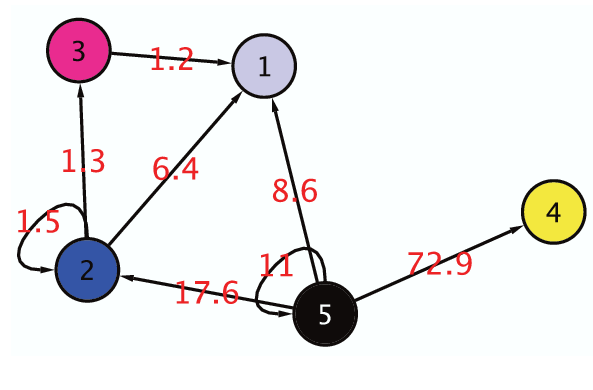
\includegraphics[scale=0.25] {TRN_Q5_summary.png} &
\vspace{0cm}
 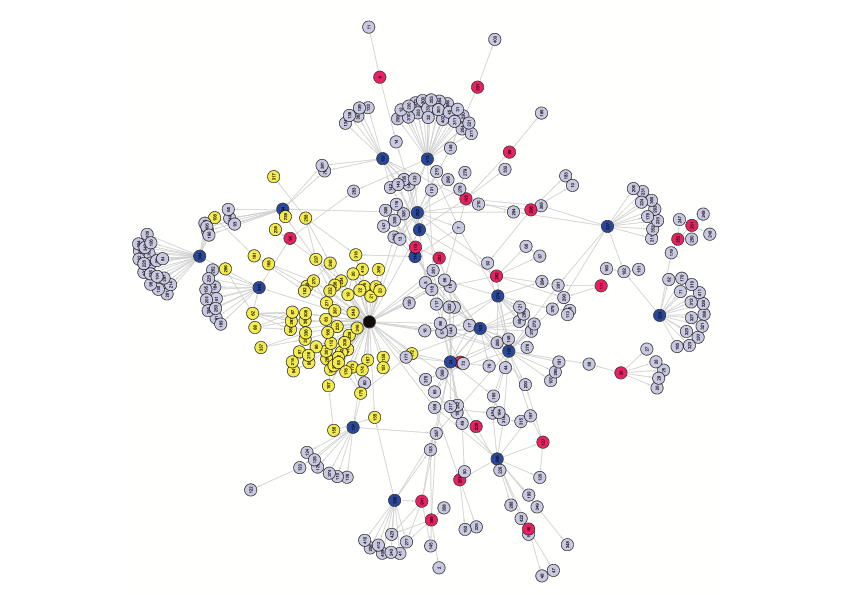
\includegraphics[scale=0.2] {Colinet_Q5.png}
   \\
  { \tiny
   \begin{tabular}{|r|rrrrr|}
  \hline
 & \multicolumn{5}{c|}{MixNet Classes} \\
 & 1 & 2 & 3 & 4 & 5 \\
  \hline
1       &   .   &   .   &   .   &   .   &   .   \\
2       & 6.40  & 1.50  & 1.34  &   .   &   .   \\
3       & 1.21  &   .   &   .   &   .   &   .   \\
4       &   .   &   .   &   .   &   .   &   .   \\
5       & 8.64  & 17.65 &   .   & 72.87 & 11.01 \\
\hline
alpha   & 65.49 & 5.18  & 7.92  & 21.10 & 0.30  \\
   \hline
\end{tabular} }
&  Meta Hierarchical structure, Meta Single Input Modules and Feed Forward Loops. \\
\end{tabular}
\end{frame}

\section{Estimation}

\begin{frame}
 \frametitle{Log-Likelihood for Mixnet}
 \begin{itemize}
 \item \textbf{Extended Log-Likelihood}
   \[
   \mathcal{L}(X,Z) = \sum_i \sum_q Z_{iq}\ln{\alpha_q} +
   \sum_{i <\ne j}
   \ln{b(\pi_{z_iz_j},X_{ij})}
   \]
   with $b(\pi_{ql},X_{ij}) = \pi_{ql}^{X_{ij}}
   (1-\pi_{ql})^{(1-X_{ij})}$

 \item \textbf{Log-Likelihood}
   \[
   \mathcal{L}(X) = \ln{\sum_{Z} \exp{\mathcal{L}(X,Z)}}
   \]

 \item $\sum$ with $Q^n$ terms: \alert{impossible}
 \item  EM algorithm: impossible to compute
   $\Pr(Z|X)$ for $(Z_i \; i=1:n)$ are not independent (conditionally to $X$).
 \end{itemize}
\end{frame}


\begin{frame}
 \frametitle{Variational Estimates}
 \textbf{Idea} Replace \alert{complicated} $\Pr(Z|X)$ by  \alert{simple} $R_X(Z)$ so that
 $KL(R_X(Z), \Pr(Z|X))$ is minimum.\bigskip

 \begin{itemize}
 \item Find $R$ which maximizes $\mathcal{J}(R)$ :
   \begin{eqnarray*}
     \mathcal{J}(R_X(Z))  & = & \mathcal{L}(X)  - KL(R_X(Z),
     \Pr(Z|X)) \\
     & = & \mathcal{H}(R_X(Z)) + \sum_{Z} R_X(Z)  \mathcal{L}(X,Z)
   \end{eqnarray*}

 \item If  $R$ is simple, $\mathcal{J}(R_X(Z))$ can be computed. For Mixnet  $R_X(Z)\in \mathcal{F}$ with $\mathcal{F}=\left\{ f:f(Z)=\prod_{i=1}^nf_i(Z_i)\right\}$ \bigskip
 \item At best , $R_X(Z) = \Pr(Z|X)$ and $\mathcal{J}(R_X(Z))
   = \mathcal{L}(X)$.
 \end{itemize}
\end{frame}

\begin{frame}
\frametitle{What is known about the quality of variational estimates?}
\begin{itemize}
\item
Gunawardana and Byrne (JMLR 2002): the variational estimates are consistent only for degenerate cases.
\item  consistent in some cases (simple mixtures, some latent variable models and Markovian model)
\item not consistent in some other ones (state space model).
\item simulations show that variational estimates are consistent for Mixnet model
\end{itemize}
\end{frame}

\begin{frame}
\frametitle{Results}
\begin{description}
\item [Degeneracy] Mixnet is degenerate ($P(Z/X) \rightarrow \text{Dirac}$) when the number of vertices approaches infinity
\item [New semi-parametric model] A new semi-parametric model can be defined which contains $n*c$ parameters ($n$ is the number of vertices and $c$ is a constant) and $n^2$ observations. In this non standard asymptotic framework, the maximum likelihood estimates are consistent.
\item [Asymptotic equivalence] The variational and maximum-likelihood estimates are asymptotically equivalent $ \Rightarrow$ the variational estimates are consistent
\end{enumerate}
\end{frame}

\section{Degeneracy of Mixnet}


\begin{frame}
\frametitle{Concentration for $P(Z/X)$}
$\P(Z=z \mid X)=\frac{P(X\mid Z=z)P(Z=z)}{P(X)}$ is a random variable depending on $X$.
\begin{theorem}
Condition C1: \hspace{1cm}   $\forall (q \ne q') \; \; \;
\exists l \in (1,Q) \; : \; \pi_{ql} \ne \pi_{q'l}$ or $\pi_{lq} \ne \pi_{lq'}$ \\
Condition C2: \hspace{1cm} \exists a>0 \; : \; $\min_{1>\pi_{ql}>0}(\pi_{ql},(1-\pi_{ql}))>a$ \\
Condition C3: \hspace{1cm} \exists b>0 \; : \; $\min_q  \alpha_{q} >b$ \\
Assume that conditions C1,C2 and C3 are true. Then when $n \rightarrow \infty$

$$ \forall t>0,  \;  \P_{X|Z=z^*} \left[ \frac{ \P(Z \ne z^* \mid X) }{ \P(Z=z^*\mid X)} >t \right] \rightarrow 0$$

\end{theorem}
\begin{block}{Corollary}
$  \Rightarrow \mathcal{L}(\P_{X|Z=z^*}(Z \mid X)) \rightarrow \delta (z^*)$ when $n \rightarrow \infty $
\end{block}
\end{frame}

\begin{frame}
\frametitle{Outline of proof}
\begin{itemize}
  \item $\P(Z=z \mid X)=\frac{P(X\mid Z=z)P(Z=z)}{P(X)}$ is a random variable depending on $X$,
  \item the ratio $\frac{ \P(Z \ne z^* \mid X) }{ \P(Z=z^*\mid X)}$ eliminates the problematic $P(X)$,
  \item $P(X\mid Z=z)P(Z=z)=\prod_{i\neq j} \pi_{z_iz_j}^{x_{ij}}(1-\pi_{z_iz_j})^{(1-x_{ij})}\prod_{i} \alpha_{z_i}\Rightarrow \log \left[\frac{ \P(Z = z \mid X) }{ \P(Z=z^*\mid X)}\right]$ is a sum of $an^2$ terms
  \item Bernstein inequality implies that the speed of concentration of the above function to its mean is of order $n^2$,
  \item $\P(Z \ne z^* \mid X)=\sum_{z \neq z^*} P(Z=z \mid X)$ is a sum of $Q^n=e^{n\log Q}$ terms,
  \item $n^2$ wins against $n$.
\end{itemize}



\end{frame}


\section{Consistency for Mixnet-FP}

\begin{frame}
\frametitle{Mixnet-FP: semi-parametric model}
{\bf Mixnet with fixed parameters for each node.}


\begin{itemize}
\item $i=1,\ldots,n$ vertices \item $q=1,\ldots,Q$ classes \item $X_{ij}=1$ if
there is an edge from node $i$ to node $j$.
 \item
$\zn \in \Z_{[n]}=(1,Q)^{n}$
 \item $X_{ij}$ are independent Bernoulli RV with
       $\P(X_{ij}=1)=\pi_{z_iz_j},$
       \item Mixnet-FP parameters: $\zn, \pi$
\end{itemize}
\alert {Non-standard asymptotic framework}:
 \begin{itemize}
   \item the vector of parameters $\zn$ depends on $n$,
   \item its dimension is equal to $n$,
   \item $n^2$ observations $X_{[n]}$
 \end{itemize}

\end{frame}

\begin{frame}
\frametitle{Mixnet-FP(M1): results}
\begin{description}
  \item [Identifiability] Under condition C1, for every $n$, the model M1 is identifiable: let $\theta_n=(\zn,\pi)$,
 $$\P_{\theta_n}(.)=\P_{\theta_n'}(.) \Rightarrow \theta_n=\theta_n'$$
  \item [Empirical likelihood]
$\L_1\paren{\xn;\theta_n}=\sum_{i,j \neq i} b_{ij}(z_i,z_j),$ with $b_{ij}(q,l)=x_{ij}\log\pi_{ql}+(1-x_{ij})\log(1-\pi_{ql}).$
\item [Consistency]
For every $n\in\N^*$, let $\Theta_n\subset\Theta$ denote a metric space endowed with a distance $d(\cdot,\cdot)$. Assume that conditions C1 and C2 are true,
let $\theta_n^*$ be the true parameter and $\widehat{\theta}_n$ the ML estimate, then
$d\paren{\widehat{\theta}_n,\theta_n^*}\xrightarrow[n\to+\infty]{P^*}0\enspace.$
\end{description}



\end{frame}


\begin{frame}
\frametitle{Outline of proof}
The reference probability is $P^*=\P\croch{\cdot\mid Z=z^*}$
\begin{description}
  \item [Normalized Empirical Likelihood] 
  \begin{align*}
        M_n\paren{\theta_n} & \defegal \frac{1}{n(n-1)} \L_1\paren{\xn;\theta_n},\\
        \mathbb{M}_n\paren{\theta_n}&\defegal \E^*\croch{M_n\paren{\zn,\theta_n}}=\E^*\croch{M_n\paren{\zn,\theta_n}\mid Z=z^*}\enspace.
\end{align*}
  \item [Consistency for M-estimates in a metric space]
  \begin{thm} \label{thm.conv.proba.theta.hat}
For every $n\in\N^*$, let $\Theta_n\subset\Theta$ denote a metric space endowed with a distance $d(\cdot,\cdot)$. Let us further assume that the following assumptions hold:
\begin{enumerate}
        \item $\forall n\in\N^*,\quad \sup_{d(\theta,\theta_n^*)>\delta } \mathbb{M}_n(\theta)<\mathbb{M}_n(\theta_n^*)$,
        \item $\norm{M_n-\mathbb{M}_n}_{\Theta_n}\xrightarrow[n\to +\infty]{P^*}0$.
\end{enumerate}
Then, $M_n(\widehat{\theta}_n)\geq \sup_{\theta\in\Theta_n}M_n\paren{\theta}+o_{P^*}(1)$ implies that
\begin{align*}
        d\paren{\widehat{\theta}_n,\theta_n^*}\xrightarrow[n\to+\infty]{P^*}0\enspace.
\end{align*}
\end{thm}
  \item [Uniform convergence] Concentration inequalities (Talagrand)
\end{description}



\end{frame}

\section{Consistency of variational estimates for Mixnet}
\begin{frame}
\frametitle{Notations for Mixnet(M2)}
\begin{description}
\item[Parameters]
$\alpha^*$: true value of $\alpha$, $\pi^*$: true value of $\pi$.

\item[Variational likelihood approximation]
$$\J(\xn; \taun, \pi, \alpha)= $$ $$\sum_{i,j \neq i} \sum_{ql} b_{ij}(q,l)\tau_{iq}\tau_{jl}-\sum_{iq}\tau_{iq}\log\tau_{iq}+\sum_{iq}\tau_{iq}\log\alpha_{q}$$

\item[Likelihood]
 $$\L_2(\xn; \alpha,\pi)= \log \left\{ \sum_{z_{[n]} \in \Zdefn} e^{\left[ \sum_{i,j \neq i}^n b_{ij}(z_i,z_j) \right]} P_{\Zn}(\zn) \right\}$$

\item[$\znt$]

$\znt=\znt(\pi,\xn)=\argmax_{\zn} \L_2(\xn; \alpha,\pi)$

\item[$\tah$]

$\tah=\tah(\pi,\xn)=\argmax_{\taun} \J(\xn; \taun,\pi,\alpha)$ with $\tau \in S_n$, with $S_n=\{u \in ([0,1]^Q)^n \; : \; \forall i=1:n, \; \; \sum _{q=1}^Q u_{iq}=1 \}$
\end{description}

\end{frame}

\begin{frame}
\frametitle{Results for M2}

\begin{description}
\item[$K(R_{X_n},P^{\Xn})$]

\begin{thm} For every $n$, let $\mathcal{P}_n$ denote the set of product disributions over $\mathcal{Z}_n$, and $P^{\Xn}\paren{\cdot}$ the distribution of $\Zn$ conditional to $\Xn$. Then,
\begin{align*}
K(R_{X_n},P^{\Xn})\defegal \inf_{D\in\mathcal{P}_n} K(D,P^{\Xn}) \xrightarrow[n\to\infty]{}0\enspace,\qquad P^*-a.s. \enspace.
\end{align*}
\end{thm}

\item[Consistency]
\begin{thm}\label{thm.consist.Var}
Assume that the MLE estimator $\widehat{\theta}_{\mathrm{MLE}}$ is consistent to estimate $\theta^*$, and satisfies the assumptions required for the consistency of the M-estimators. Let $\widetilde{\theta}_{n}=\arg\max_{\theta} \J(\xn; \tah, \pi, \alpha).$
Then, under C1, C2 and C3:
\begin{align*}
\mathrm{dist}\paren{\widetilde{\theta}_{n},\theta^*} \xrightarrow[n\to \infty]{P}0\enspace.
\end{align*}
\end{thm}
\end{description}
\end{frame}


\begin{frame}
\frametitle{Proof elements}


\begin{block}{Likelihoods inequalities}

For every $\xn\in\Xdefn$, $(\pi,\alpha) \in \Theta$, and $\taun \in S_n$:

$
\J(\xn; \znh, \pi, \alpha) \le \J(\xn; \tah, \pi, \alpha) \le \L_2(\xn;  \pi, \alpha) \le  \L_1(\xn; \znh,\pi)\enspace. 
$
\end{block}

 Proof of the last $\le$
\begin{eqnarray*}
% \nonumber to remove numbering (before each equation)
\L(\xn;  \pi, \alpha) &=& \log \left\{ \sum_{\zn \in \Zdefn} e^{\left[  \L(\xn; \zn,\pi) \right]} P_{\Zn}(\zn) \right\} \\
 & \le & \log \left\{ \sum_{z_{[n]} \in \Zdefn} e^{\left[  \L(\xn; \znh,\pi) \right]} P_{\Zn}(\zn) \right\} \\
 & \le & \log \left\{ e^{\left[  \L(\xn; \znh,\pi) \right]}  \sum_{z_{[n]} \in \Zdefn}  P_{\Zn}(\zn) \right\} \\
 & \le & \L(\xn; \znh,\pi)
 \end{eqnarray*}

\end{frame}

\section{Conclusions}
\begin{frame}
\frametitle{Practical conclusions}

\begin{itemize}
  \item A new asymptotic framework with an infinite parameter dimension is available for statistical models for networks
  \item The variational estimation procedure is validated
  \item One can learn exactly the group of each node for large networks and moderate $Q$.
  \item Some work to do for $Q$ depending of $n$.
\end{itemize}


\end{frame}

\end{document}










%********************************************************************








\section{Consistency of VEM estimates for Mixnet}


\begin{frame}
\frametitle{$KL(R_{X_n},P_{Z/X_n}) \rightarrow 0$ ($n\rightarrow\infty$)}

\begin{theorem}
$KL(R_{X_n},P_{Z/X_n}) \rightarrow 0$ when $n \rightarrow \infty$.
Let $(\pi, \alpha)$ be the true parameters, then $\lim_{n\rightarrow\infty} I_n-J_n =0$, with $I_n=\mathcal{L}(X_n,\pi,\alpha)$ and $J_n=\mathcal{J}(X_n,\pi,\alpha).
\end{theorem}
\begin{block}{Proof}
$\Omega=(1,Q)^{\mathbb{N}}$ suites infinies d'entiers compris entre 1 et Q, $z \in \Omega$

$\Omega_n=(1,Q)^{n}$ suites � $n$ �l�ments d'entiers compris entre 1 et Q, $z_{[n]} \in \Omega_n$

$\mathcal{A}=\mathcal{P}(\Omega)$ tribu des parties de $\Omega$, $\mathcal{A}_n=\mathcal{P}(\Omega_n)$ tribu des parties de $\Omega_n$

$z_{[n]} \in \mathcal{A}$ et $\Omega_n \in \mathcal{A}$ par r�union d'�l�ments de $\Omega$.

$(\Omega,\mathcal{A},P)$ espace probabilis� sur $\Omega$, $(\Omega_n,\mathcal{A}_n,P_n)$ espace probabilis� sur $\Omega_n$

$(\Omega_n,\mathcal{A}_n,P_{[n]})$ projection de $(\Omega,\mathcal{A},P)$ sur $\Omega_n$
avec $P_{[n]}(z_{[n]})\doteq \sum P(z)$ o� la somme est faite sur les $z$ ayant les m�mes $n$ premi�res coordonn�es que $z_{[n]}$.
\end{block}
\end{frame}


\begin{frame}
\frametitle{$KL(R_{X_n},P_{Z/X_n}) \rightarrow 0$ ($n\rightarrow\infty$) (suite)}
\begin{block}{Proof (suite)}

$$KL(P_{[n]},P_n)=\sum_{z_{[n]}}P_{[n]}(z_{[n]})\log \frac{P_{[n]}(z_{[n]})}{P_{n}(z_{[n]})}$$

$P=\delta_{z^*}$ et $P_n=P_{Z/X_n}$ :  $$KL(\delta_{z^*[n]},P_{Z/X_n})=-\log {P_{Z/X_n}(z^*_{[n]})} \rightarrow 0 (n\rightarrow \infty)$$

$\forall n, \; \;  KL(R_{X_n},P_{Z/X_n}) \le KL(\delta_{z^*[n]},P_{Z/X_n})$
 o� $R_{X_n}$ est la loi approch�e de $Z/X_n$ dans le cadre variationnel.


$$0 \le \lim_{n\rightarrow\infty} KL(R_{X_n},P_{Z/X_n}) \le \lim_{n\rightarrow\infty} KL(\delta_{z^*[n]},P_{Z/X_n})=0$$

Donc les $\tau$ variationnels tendent vers $z^*$ et d'autre part  comme

$J_n=I_n- KL(R_{X_n},P_{Z/X_n})$, on a

$$\lim_{n\rightarrow\infty} (J_n-I_n)=0$$
$\blacksquare$
\end{block}
\end{frame}

\begin{frame}
\frametitle{Inequalities between log-likelihoods}
\begin{itemize}

\item
$B_{ij}(q,l)=X_{ij}\log\pi_{ql}+(1-X_{ij})\log(1-\pi_{ql}) $

\item
Mixnet-FP loglikelihood: $\L(\xn; \zn, \pi)= \sum_{i,j \neq i} b_{ij}(z_i,z_j)$

\item
Mixnet variationnal likelihood approximation:
$$\J(\xn; \taun, \pi, \alpha)= \sum_{i,j \neq i} \sum_{ql} b_{ij}(q,l)\tau_{iq}\tau_{jl}-\sum_{iq}\tau_{iq}\log\tau_{iq}+\sum_{iq}\tau_{iq}\log\alpha_{q}$$

\item
Mixnet likelihood: $\L(\xn; \alpha,\pi)= \log \left\{ \sum_{z_{[n]} \in \Zdefn} e^{\left[ \sum_{i,j \neq i}^n b_{ij}(z_i,z_j) \right]} P_{\Zn}(\zn) \right\}$

\item
$\znh=\znh(\pi,\xn)=\argmax_{\zn} \L(\xn; \zn,\pi)$


\item
$\th=\th(\pi,\xn)=\argmax_{\taun} \J(\xn; \taun,\pi,\alpha)$ with $\taun \in S_n$, and $S_n=\{u \in ([0,1]^Q)^n \; : \; \forall i=1:n, \; \; \sum _{q=1,Q}u_{iq}=1 \}$
\end{itemize}
\end{frame}

\begin{frame}
\frametitle{Inequalities between log-likelihoods(2)}
{\bf Proposition} \\
 $ \forall \xn \in \Xdefn,(\pi,\alpha) \in \Theta, \taun \in S_n$
$$ \J(\xn; \taun, \pi, \alpha) \le \L(\xn;  \pi, \alpha) \le  \L(\xn; \znh,\pi) $$
 {\bf Proof} \\
First inequality. Definition of $ \J(\xn; \taun, \pi, \alpha)$:
    $\L(\xn;  \pi, \alpha) = \J(\xn; \taun, \pi, \alpha) + KL(Q_{\taun}(\Zn),P(\Zn/\Xn=\xn))$ \\
with $Q_{\taun}(\zn)$  any pdf of $Z$.
\begin{eqnarray*}
% \nonumber to remove numbering (before each equation)
  KL(Q_{\tau}(Z),P(Z/X=x)) &=& \sum_{z \in Z}Q_{\tau}(z)\log \left[\frac{Q_{\tau}(z)}{P(z/X=x)} \right] \\
   &=& \sum_{z \in Z}Q_{\tau}(z)\log Q_{\tau}(z)-\sum_{z \in Z}Q_{\tau}(z)\log P(z/X=x)
   \end{eqnarray*}
 \begin{eqnarray*}
   &=& \sum_{z \in Z}Q_{\tau}(z)\log Q_{\tau}(z)-\sum_{z \in Z}Q_{\tau}(z)\log P(z/X=x)P(x)+L(x,\pi,\alpha)  \\
   &=& - \J(x; \tau, \pi, \alpha)+ L(x,\pi,\alpha)
\end{eqnarray*}
 $Q_{\tau}(z)=\prod_{i=1,n}\tau_{iz_i}.$
\end{frame}

\begin{frame}
\frametitle{Inequalities between log-likelihoods(3)}
Second inequality
\begin{eqnarray*}
% \nonumber to remove numbering (before each equation)
\L(\xn;  \pi, \alpha) &=& \log \left\{ \sum_{z_{[n]} \in \Zdefn} e^{\left[ \sum_{i,j \neq i}^n b_{ij}(z_i,z_j) \right]} P_{\Zn}(\zn) \right\} \\
 & \le & \log \left\{ \sum_{z_{[n]} \in \Zdefn} e^{\left[ \sum_{i,j \neq i}^n b_{ij}(\zh_i,\zh_j) \right]} P_{\Zn}(\zn) \right\} \\
 & \le & \log \left\{ e^{\left[ \sum_{i,j \neq i}^n b_{ij}(\zh_i,\zh_j) \right]}  \sum_{z_{[n]} \in \Zdefn}  P_{\Zn}(\zn) \right\} \\
 & \le & \L(\xn; \znh,\pi)
 \end{eqnarray*}
\end{frame}

\begin{frame}
\frametitle{Inequalities between log-likelihoods(4)}
Consequence of the above inequalities :

 $ \forall \xn \in \Xdefn,(\pi,\alpha) \in \Theta $ :

$$ \J(\xn; \znh, \pi, \alpha) \le  \J(\xn; \tnh, \pi, \alpha) \le \L(\xn;  \pi, \alpha) \le  \L(\xn; \znh,\pi). $$
Moreover $$\J(\xn; \znh, \pi, \alpha)= \L(\xn; \znh,\pi)+\sum_i \log \alpha_{\zh_i}.$$

\end{frame}

\begin{frame}
\frametitle{Inequalities between log-likelihoods(5)}
$$   \sum_i \log \alpha_{\zh_i} \le  \J(\xn; \tnh, \pi, \alpha)-\L(\xn; \znh,\pi) \le \L(\xn;  \pi, \alpha)-\L(\xn; \znh,\pi) \le  0. $$
Let $\epsilon =\min_q(\alpha_q) >0$.

Then  $ \forall \xn \in \Xdefn,(\pi,\alpha) \in \Theta $

$$   \frac{1}{n(n-1)}|\L(\xn;  \pi, \alpha)-\L(\xn; \znh,\pi)|  $$
$$ \le \frac{1}{n(n-1)} |\J(\xn; \tnh, \pi, \alpha)-\L(\xn; \znh,\pi)|$$
$$ \le \frac{-\log \epsilon}{n-1}. $$
\end{frame}



\begin{frame}
\frametitle{Consistency of VEM estimates}

\begin{theorem}
Assume that conditions C1' and C3 are true. Let $\widehat{\theta}_n$ and $\widetilde{\theta}_n$ be respectively the ML and variational estimates of the Mixnet parameter $\theta_0$. Then $\lim_{n \rightarrow \infty}(\widehat{\theta}_n-\widetilde{\theta}_n)=  0$ in probability.
\end{theorem}
\begin{block}{Proof}
$\mathcal{L}_{\infty}(\theta)=\lim_{n \rightarrow\infty}\frac{1}{n^2}\mathcal{L}(\theta,X)$ and  $\mathcal{J}_{\infty}(\theta)=\lim_{n \rightarrow\infty}\frac{1}{n^2}\mathcal{J}(\theta,X)$

$\theta_0=\arg\max_{\theta}\mathcal{L}_{\infty}(\theta)$ and $\theta_1=\arg\max_{\theta}\mathcal{J}_{\infty}(\theta)$.


$\lim_{n \rightarrow \infty}(\widehat{\theta}_n-\theta_0)=  0$ and $\lim_{n \rightarrow \infty}(\widetilde{\theta}_n-\theta_1) = 0$ in probability,


$   P_\infty(Z|X)=\delta_{z^*}(Z)$

\framebox{Property of the multivariate Dirac distribution:
$\delta_{z^*}(Z)=\prod_{i=1}^n \delta_{z^*_i}(Z_i)$}  remains true when $n\rightarrow \infty$ \\


$\Rightarrow P_{\infty}(Z \mid X) \in \mathcal{F}$ $\Rightarrow R_{X\infty} = P_{\infty}(Z|X)$ and $\mathcal{J}_{\infty}
   = \mathcal{L}_{\infty}$.\\


   $\mathcal{J}_{\infty} = \mathcal{L}_{\infty} \Rightarrow \theta_0=\theta_1 \Rightarrow \widehat{\theta}_n-\widetilde{\theta}_n= \widehat{\theta}_n-\theta_0-(\widetilde{\theta}_n-\theta_1) \Rightarrow \lim_{n\rightarrow\infty}\widehat{\theta}_n-\widetilde{\theta}_n=0$.
   $\blacksquare$
\end{block}
\end{frame}

\section{Consistency of ML Estimates for MixnetFP} \label{Sec:Convergence}


\begin{frame}
\frametitle{Model MixnetFP}


$\mathcal{A}= \left\{ z=(z_1,...z_i...), \; z_i \in (1,Q) \right\}$ set of (non random) infinite sequences of non-null integers $ \le Q$.

$\mathcal{A}_n \subset \mathcal{A}$  set
of the $n$ first elements, $z_{[n]}$ of $z \in \mathcal{A}$.

\begin{block}{Model}
\begin{itemize}
\item$i=1,n$ nodes
\item $q=1,Q$ classes
\item $X_{ij}=1$ if there
is an edge from node $i$ to node $j$
\item $z^*_{[n]} \in
\mathcal{A}_n$ and $\pi^* \in [0,1]^{Q^2}$. Condition C1' is assumed in order to obtain
identifiability :$\forall (q \ne q') \; \; \;
\exists l \in (1,Q) \; : \; \pi_{ql} \ne \pi_{q'l}$ or $\pi_{lq} \ne \pi_{lq'}$

\item $X_{ij}$ are independent Bernoulli RV with
$P(X_{ij}=1)=\pi^*_{z^*_iz^*_j}$
\end{itemize}
\end{block}
\end{frame}

\begin{frame}
\frametitle{Conditions C1', C2 }
\begin{block}{Condition C1'}
   $\forall (q \ne q') \; \; \;
\exists l \in (1,Q) \; : \; \pi_{ql} \ne \pi_{q'l}$ or $\pi_{lq} \ne \pi_{lq'}.$
\end{block}
\begin{block}{Condition C2 (no empty class)}
$\forall q \in (1,Q) \; \; \; \exists i \in (1,n) \; : \; z_i=q.$
\end{block}
\end{frame}

\begin{frame}
\frametitle{Identifiability of Mixnet-FP under C1'and C2 }
\begin{itemize}

 \item $P$  matrix : $\forall (i,j) \; \; P_{ij}= \pi_{z_i z_j}$
 \item $P_i$ : line $i$ of $P$
 \item $\pi_q$  line $q$ of  $\pi$. \\
 \item Any element of $P_i$ is a member of the set of the elements of $\pi_{z_i}$ and by C2 all the elements of $\pi_{z_i}$  are present in $P_i$
 \item same property for columns
 \item
  if $z_i \neq z_j$ then the $i^{th}$ and $j^{th}$ lines or columns of $P$ are different.
 \item if $z_i = z_j$ then the $i^{th}$ and $j^{th}$ lines or columns of $P$ are equal.
 \end{itemize}
 \end{frame}

\begin{frame}
\frametitle{Identifiability of Mixnet-FP under C1'and C2(2) }
 \begin{itemize}

 \item
 equivalence relation $i \sim j \Leftrightarrow z_i=z_j \Leftrightarrow (P_i=P_j) \cap (P'_i=P'j)$
  \item $Q$ equivalence classes
 \item
 Let  $(Z^{(1)},\pi^{(1)})$ such that $\forall (i,j) \; \; P_{ij}= \pi^{(1)}_{z^{(1)}_i z^{(1)}_j}$
 \item
  Equivalence relation  based on $P$ $\Rightarrow $ also true for $Z^{(1)}$
  \item
 equivalence classes are the same for $Z^{(1)}$ and $Z$
 \item
 The only difference are the labels $(1,2,...Q)$ of the classes
 \item
 $\sigma$ a permutation on $(1,Q)$.  Only possible couples $(Z^{(1)},\pi^{(1)})$  defined by $Z^{(1)}=Z \circ \sigma$ with $\pi^{(1)}_{ql}=\pi_{\sigma^{-1}(q),\sigma^{-1}(l)}$
 \item
 Finally $(Z,\pi)$ is unique, free from permutations.
 \end{itemize}
\end{frame}

\begin{frame}
\frametitle{Consistency of ML estimates}

\begin{equation}\label{LL}
\mathcal L(X_n, z_{[n]},\pi)= \sum_{i,j \neq i}^n  \left[ X_{ij} \ln \pi_{z_iz_j} + (1-X_{ij}) \ln (1-\pi_{z_iz_j}) \right] \end{equation}

The parameters of the model $(z,\pi)$ live in the set $\mathcal{B}=(\mathcal{A} \times[0,1]^{Q^2})$.

\begin{theorem} \label{th3}

Let $\widehat{\theta}\defegal(\widehat{z_n},\widehat{\pi})=
\argmax_{(z_{[n]},\pi) \in\mathcal{B}} \mathcal L(X_n, z_{[n]},\pi)
$,
 the maximum likelihood estimate of \hspace{0.2cm} $\theta_0\defegal(z^*_{[n]},\pi^*)$.
 Then
$
\norminf{\widehat{\theta}-\theta_0}%(\widehat{z}_n,\widehat{\pi})
%- (z^*_{[n]},\pi^*)
\xrightarrow[n\to\infty]{P} 0 $.
\end{theorem}

\end{frame}

\begin{frame}
\frametitle{Proof(1)}
\begin{lemma} \label{VDV} (Van der Vaart, p287) Let $Y_1...Y_n$ be random variables depending of a vector of parameters $\theta$
pertaining to a metric space such that:
\begin{enumerate}
 \item  for all neighborhood $G$ of $\theta_0$ and $ \forall \theta \notin G$,   $E\left[
 \mathcal L(Y_1...Y_n,\theta_0)\right]>E\left[ \mathcal L(Y_1...Y_n,\theta)) \right]$,
 \item $\frac{1}{n} \mathcal L(Y_n, \theta)- E \left[ \frac{1}{n} \mathcal L(Y_n,\theta) \right] \xrightarrow{P}
 0$  uniformly in $\theta$ when $n \rightarrow \infty$.
\end{enumerate}
Then  $ \widehat{\theta} \xrightarrow{P} \theta_0$ when $n
\rightarrow \infty$.
\end{lemma}

\end{frame}
\begin{frame}
\frametitle{Proof(2): condition 1 of Lemma}
$V_{ij}^{z_iz_j}=X_{ij} \ln \pi_{z_iz_j}+(1-X_{ij}) \ln {1- \pi_{z_iz_j}}$, \\[0.2cm]
$E(V_{ij}^{z_iz_j})= \pi^*_{z^*_iz^*_j} \ln \pi_{z_iz_j} + (1-\pi^*_{z^*_iz^*_j}) \ln (1-\pi_{z_iz_j})$.\\[0.2cm]


$\mathcal L(X_n, z_{[n]},\pi)= \sum_{i,j \neq i}^n V_{ij}^{z_iz_j}  $\\[0.4cm]


$E \left[ \mathcal L(X_n, z_{[n]},\pi) \right]= \sum_{i,j \neq i}^n \pi^*_{z^*_iz^*_j} \ln \pi_{z_iz_j} + (1-\pi^*_{z^*_iz^*_j}) \ln (1-\pi_{z_iz_j})$\\[0.2cm]

$E \left[ \mathcal L(X_n, z^*_{[n]},\pi^*) \right]= \sum_{i,j \neq i}^n \pi^*_{z^*_iz^*_j} \ln \pi^*_{z^*_iz^*_j} + (1-\pi^*_{z^*_iz^*_j}) \ln (1-\pi^*_{z^*_iz^*_j}) $ \\[0.4cm]



$E \left[ \mathcal L(X_n, z^*_{[n]},\pi^*) \right] -E \left[ \mathcal L(X_n, z_{[n]},\pi)\right]= \sum_{i,j \neq i}^n \pi^*_{z^*_iz^*_j} \ln \frac{\pi^*_{z^*_iz^*_j}}{\pi_{z_iz_j}} + (1-\pi^*_{z^*_iz^*_j}) \ln \frac{(1-\pi^*_{z^*_iz^*_j})}{(1-\pi_{z_iz_j})}$

\end{frame}

\begin{frame}
\frametitle{Proof(3): condition 1 of Lemma(2)}
\framebox{$E \left[ \mathcal L(X_n, z^*_{[n]},\pi^*) \right]-E \left[ \mathcal L(X_n, z_{[n]},\pi) \right]=
\sum_{i, j \neq i}^n KL \left[
\mathcal{B}_{ij}(z^*,\pi^*),\mathcal{B}_{ij}(z,\pi)
\right]$}\\[0.3cm]

$\mathcal{B}_{ij}(z,\pi)$ : Bernoulli pdf with parameter $\pi_{z_iz_j}$\\[0.4cm]
\begin{itemize}
  \item if $z \neq z^*$ at least one vertex is not in the same group using $z$ or $z^*$, so that the above difference is strictly positive for any $\pi$.
  \item  if $z=z^*$ and $\min | \pi-\pi^* | > \eps$, this difference is also positive.
\end{itemize}

\end{frame}


\begin{frame}
\frametitle{Proof(4): condition 2 of Lemma}
Let $(\pi^*,z^*)$ : true vector of parameters, $(\pi,z)$ : current vector of parameters.   Mixnet-FP normalized log-likelihood :
$$ \mathcal L(X_n,\pi,z) = \frac{1}{n(n-1)}\sum_{i \neq j} \left[ X_{ij} \log \pi_{z_iz_j} + (1-X_{ij}) \log (1-\pi_{z_iz_j})\right] $$
Let
  $$f(\pi,z)=E\left[ \mathcal L(X_n,\pi,z)\right] =  \frac{1}{n(n-1)}
   \sum_{i \neq j} \left[ \pi^*_{z^*_iz^*_j} \log \pi_{z_iz_j} + (1-\pi^*_{z^*_iz^*_j}) \log (1-\pi_{z_iz_j}) \right] $$ and
   $$M(X_n,z,\pi)=\mathcal L(X_n,\pi,z)-f(\pi,z) = \frac{1}{n(n-1)}\sum_{i \neq j} \left[ (X_{ij}-\pi^*_{z^*_iz^*_j}) \log \frac{\pi_{z_iz_j}}{1-\pi_{z_iz_j}} \right]  $$
\end{frame}

\begin{frame}
\frametitle{Proof(5): condition 2 of Lemma}
\begin{description}
  \item[C1] $\pi^*_{z^*_iz^*_j} > 0 \Rightarrow \pi_{z_iz_j} > 0$, and  $\pi^*_{z^*_iz^*_j} < 1 \Rightarrow \pi_{z_iz_j} < 1 $,

       for if $\pi_{z_iz_j}=(0,1)$ and $\pi_{z_iz_j} \ne \pi^*_{z^*_iz^*_j}$,  $\mathcal L(X_n,\pi,z_n)$ may be $<-\infty$ the vector of parameters $(\pi,z)$ is not admissible.
  \item[C2] $\min (\pi_{ql} \; : \; \pi_{ql} > 0) > \eps$ \hspace{1cm} and \hspace{1cm} $\min( 1-\pi_{ql} \; : \; \pi_{ql} <1 ) > \eps.$
  \item[C3] Let $A_{q,n}(z)= \left \{i=1,n, \; z_i=q  \right \}$ and $N_{q,n}(z)=\# A_{q,n}$ and $\alpha>0$. Then $ \forall z, \exists n_0 : \; n>n_0 \Rightarrow N_{q,n}(z)) > \alpha n.$
\end{description}
Let  $ \Theta(\pi^*,z^*)=\left\{(\pi,z) \in [0,1]^{Q^2}\times(1,Q)^{\mathbb{N}} \;  \; \text {satisfying} \; C1, \; C2 \; and \; C3 \right\} $.

\begin{theorem}
$$ \forall t>0, \; \;  P_{(\pi^*,z^*)}\left[ \sup_{(\pi,z) \in \Theta(\pi^*,z^*)}|M(X_n,\pi,z)|>t\right] \xrightarrow[n\to\infty]{} 0.$$
\end{theorem}
\end{frame}

\begin{frame}
\frametitle{Proof(6): proof of uniform cv}
\begin{lemma}
  $$ \forall t>0, \;  P_{(\pi^*,z^*)} \left[ \left|\frac{1}{n(n-1)} \sum_{i \in A_q \; j \in A_l \;  i\neq j} (X_{ij}-\pi^*_{z^*_iz^*_j}) \right| >t \right] \le e^{-2n(n-1) \alpha^2 t^2}$$
\end{lemma}
The lemma comes from Bernstein's inequality with
$Y_{ij}=(X_{ij}-\pi^*_{z^*_iz^*_j}),$
 and
\begin{itemize}
  \item $E(Y_{ij})=0$
  \item $V(Y_{ij})=\pi^*_{z^*_iz^*_j}(1-\pi^*_{z^*_iz^*_j}) \le \frac{1}{4}$
  \item $|Y_{ij}| \le b=1$.
  \item $Y_{ij}$ are independent
\end{itemize}
\end{frame}

\begin{frame}
\frametitle{Proof(6): proof of uniform cv}
Let
$$B_{ql}(X_n,\pi,z)=\frac{1}{n(n-1)}\sum_{i \in A_q \; j \in A_l \;  i\neq j}(X_{ij}-\pi^*_{z_i^*z_j^*})\log\frac{\pi_{ql}}{1-\pi_{ql}}.$$
We have
$$M(X_n,z,\pi)=\sum_{ql}B_{ql}(X_n,\pi,z)$$ and
$$|M(X_n,z,\pi)| \le \sum_{ql}|B_{ql}(X_n,\pi,z)|$$

for fixed $z$, $$\sup_{\pi}|B_{ql}(X_n,\pi,z)| < \frac{1}{n(n-1)}\log{\frac{1-\eps}{\eps}}\left| \sum_{i \in A_q \; j \in A_l \;  i\neq j} (X_{ij}-\pi^*_{z^*_iz^*_j}) \right|.$$


$$\sup_{\pi}|M(X_n,z,\pi)| \le \frac{1}{n(n-1)}\sum_{ql}\log{\frac{1-\eps}{\eps}}\left| \sum_{i \in A_q \; j \in A_l \;  i\neq j} (X_{ij}-\pi^*_{z^*_iz^*_j})\right|$$
\end{frame}

\begin{frame}
\frametitle{Proof(7): proof of uniform cv}
Finally for a fixed $z$, $$P_{(\pi^*,z^*)} \left[ \sup_{\pi}|M(X_n,z,\pi)| >u \right]$$

\begin{eqnarray*}
% \nonumber to remove numbering (before each equation)
   & \le & P_{(\pi^*,z^*)} \left[\log{\frac{1-\eps}{\eps}}\sum_{ql}\left| \frac{1}{n(n-1)}\sum_{i \in A_q \; j \in A_l \;  i\neq j} (X_{ij}-\pi^*_{z^*_iz^*_j})\right|  >u \right] \\
   & \le & \sum_{ql} P_{(\pi^*,z^*)} \left[\left|\frac{1}{n(n-1)} \sum_{i \in A_q \; j \in A_l \;  i\neq j} (X_{ij}-\pi^*_{z^*_iz^*_j})\right|  >\frac{u}{Q^2 \log{\frac{1-\eps}{\eps}}} \right] \\
   & \le & Q^2 e^{-2n(n-1) \alpha^2 \left[ \frac{u}{Q^2 \log{\frac{1-\eps}{\eps}}} \right] ^2} \\
   & \le & e^{2 \log Q-2n(n-1) \alpha^2 \left[ \frac{u}{Q^2 \log{\frac{1-\eps}{\eps}}} \right] ^2}
\end{eqnarray*}
\end{frame}

\begin{frame}
\frametitle{Proof(8): proof of uniform cv}
The control on all the values of $z$ :
\begin{eqnarray*}
% \nonumber to remove numbering (before each equation)
P_{(\pi^*,z^*)} \left[ \sup_{\pi,z}|M(X_n,z,\pi)| >u \right] & \le &  P_{(\pi^*,z^*)} \left\{ \bigcup_z \left[\sup_{\pi}|M(X_n,z,\pi)|  >u \right] \right \}\\
   & \le & \sum_z P_{(\pi^*,z^*)}\left[ \sup_{\pi}|M(X_n,z,\pi)|  >u \right]\\
   & \le & Q^n e^{2 \log Q-2n(n-1) \alpha^2 \left[ \frac{u}{Q^2 \log{\frac{1-\eps}{\eps}}} \right] ^2}\\
   & \le & e^{(n+2) \log Q-2n(n-1) \alpha^2 \left[ \frac{u}{Q^2 \log{\frac{1-\eps}{\eps}}} \right] ^2}
\end{eqnarray*}
$\blacksquare$
\end{frame}



% Convergence simple
%\begin{block}{Chebyshev's theorem (Serfling, p. 27)}
%  $X_1, X_2, ... $ independent,  $E(X_i)=\mu_i$, \hspace{0.1cm} $V(X_i)=\sigma_i^2$, \hspace{0.1cm}
% $\sum_1^{\infty}
%\sigma_i^2=\text{o}(n^2)$
%
% then $  \frac{1}{n} \sum_{i=1}^n X_i -
%\frac{1}{n} \sum_{i=1}^n \mu_i \xrightarrow{P} 0 $ when $n
%\rightarrow \infty$.\\[0.3cm]
%\end{block}
%
%\begin{equation*}\label{LL1}
% \frac{1}{n^2} \mathcal L(X_n, z_{[n]},\pi)- E\left[ \frac{1}{n^2} \mathcal L(X_n, z_{[n]},\pi) \right] = \frac{1}{n^2} \sum_{i,j}^n  V_{ij}^{z_iz_j}  - \frac{1}{n^2} \sum_{i,j}^n  E( V_{ij}^{z_iz_j})
%\end{equation*}
%
%
%\begin{eqnarray*}
%\text{Var}( V_{ij}^{z_iz_j}) &=& \text{Var}( X_{ij} \ln \pi_{z_iz_j}  +(1-X_{ij}) \ln (1-\pi_{z_iz_j} )  )
%\\ &=& (\ln \frac{\pi_{z_iz_j}}{1-\pi_{z_iz_j}} )^2 \pi_{z_iz_j}(1-\pi_{z_iz_j} )
%\end{eqnarray*}
%
% $f(x)=\left[\log\left( \frac{x}{1-x}\right)\right]^2x(1-x) \le 0.43923$ for $x \in[0,1] \Rightarrow
%\text{Var}( V_{ij}^{z_iz_j}) \leqslant  \frac{1}{2} $
%
%
%$ \sum_{i,j} \text{Var}( v_{ij}^{z_iz_j}) \leqslant  \frac{1}{2}n^2 \sim \text{o}(n^4) $
%
%Then $ \frac{1}{n^2} \mathcal L(X_n, z_{[n]},\pi)- E(
%\frac{1}{n^2} \mathcal L(X_n, z_{[n]},\pi) )  \xrightarrow{P} 0$
%when $n \rightarrow \infty$.




\begin{frame}
\frametitle{Ranking the log-likelihoods(1)}
\begin{block}{MixnetFP}
  $\mathcal L(X, z,\pi)= \sum_{i,j \neq i}^n  \left[ X_{ij} \ln \pi_{z_iz_j} + (1-X_{ij}) \ln (1-\pi_{z_iz_j})\right]$ \end{block}
  \begin{block}{Mixnet log-likelihood}
$\mathcal L(X, \alpha,\pi)= \log\left\{ \sum_z \exp \left[ \sum_{i} \log \alpha_{z_i} +\sum_{i \neq j} \left(X_{ij} \ln \pi_{z_iz_j} + (1-X_{ij}) \ln (1-\pi_{z_iz_j})\right) \right] \right\}$ \\[0.4cm]
\end{block}
 \begin{block}{Mixnet variational log-likelihood}
 $\mathcal J(X,\alpha,\pi)= \sum_{iq} \log \alpha_{q}\tau_{iq}+\sum_{i,j \neq i}^n \sum_{ql} \left[ X_{ij} \ln \pi_{ql} + (1-X_{ij}) \ln (1-\pi_{ql})\right]\tau_{iq}\tau_{jl}-\sum_{iq}\tau_{iq}\log\tau_{iq}$ \\[0.2cm]
 $\tau$ is solution of $\sum_q\tau_{iq}=1$ and $\log\tau_{iq} \propto \log\alpha_q+\sum_{j \neq i}^n \sum_{l} \left[ X_{ij} \ln \pi_{ql} + (1-X_{ij}) \ln (1-\pi_{ql})\right]\tau_{jl} \; \; \text{for} \; i=1...n.$
\end{block}

\end{frame}

\begin{frame}
\frametitle{Ranking the log-likelihoods(2)}
\begin{itemize}
\item
$(\hat{z},\check{\pi})=\argmax_{(z,\pi) \in\mathcal{B}} \mathcal L(X, z,\pi)$
\item
$(\hat{\alpha},\hat{\pi})=\argmax_{(\alpha,\pi)} \mathcal L(X, \alpha,\pi)$
\item
$(\tilde{\alpha},\tilde{\pi})=\argmax_{(\alpha,\pi)} \mathcal J(X, \alpha,\pi)$
\end{itemize}

$$\mathcal J(X, \tilde{\alpha},\tilde{\pi}) \le \mathcal L(X, \hat{\alpha},\hat{\pi}) \le \mathcal L(X, \hat{z},\check{\pi})$$

First inequality : definition of $\mathcal J$

Second inequality:
  \begin{eqnarray*}
   & & \mathcal L(X, \hat{\alpha},\hat{\pi})\\
  % \nonumber to remove numbering (before each equation)
   &=& \log\left\{ \sum_z \exp \left[ \sum_{i} \log \hat{\alpha}_{z_i} +\sum_{i \neq j} \left(X_{ij} \ln \hat{\pi}_{z_iz_j} + (1-X_{ij}) \ln (1-\hat{\pi}_{z_iz_j})\right) \right] \right\} \\
   & \le & \log\left\{ \sum_z \exp \left[ \sum_{i} \log \hat{\alpha}_{z_i} +\sum_{i \neq j} \left(X_{ij} \ln \check{\pi}_{\hat{z_i}\hat{z_j}} + (1-X_{ij}) \log (1-\check{\pi}_\hat{z_i}\hat{z_j})\right) \right] \right\} \\
   & \le & \mathcal L(X, \hat{z},\check{\pi})
  \end{eqnarray*}

\end{frame}

\section{Worksheet}
\begin{frame}
\frametitle{Worksheet}
\begin{description}
\item[Algorithm]
Build an estimation algorithm for MixnetFP
\item[Motifs]
Usual count statistic for motif $m_k$:$$\sum_{(i_1...i_k) \in (1...n)}\left\{ \mathbb{1}(G_{i_1...i_k}=m_k) \right\} $$ needs an homogeneous model.\\[0.5cm]
MixnetFP : non-homogeneous model $\rightarrow$ a new statistic using MixnetFP:
$$\sum_{(i_1...i_k) \in (1...n)}\left\{ \frac{\mathbb{1}(G_{i_1...i_k}=m_k)-E\left[\mathbb{1}(G_{i_1...i_k}=m_k)\right]}
{E\left[\mathbb{1}(G_{i_1...i_k}=m_k)\right]\left(1-E\left[\mathbb{1}(G_{i_1...i_k}=m_k)\right]\right)} \right\} $$

\end{description}
Allows to analyse "network-localized" deviations from the expected value for motif $m_k$.


\end{frame}

\end{document}





